\documentclass{article}
\usepackage{amsmath}
\usepackage{amsfonts}
\usepackage{graphicx}
\usepackage{siunitx}

\graphicspath{./}

\newcommand{\transf}[1]{\mathcal H(#1)}
\newcommand{\freq}[1]{H(#1)}
\newcommand{\magres}[1]{|\freq{#1}|}

\begin{document}
\title{Homework 5}
\author{Edgar Jose Donoso Mansilla}
\date{}
\maketitle

\section{Inverse Comb Filter}
$$
	y_t = x_t - R^L x_{t-L},\ R = 0.999,\ L = 6
$$

\subsection{Transfer Function $\transf{z}$}
\begin{align*}
	Y          & = X(1 - R^L z^{-L})  \\
	\transf{z} & = 1 - 0.999^6 z^{-6}
\end{align*}

\subsection{Frequency Response $\freq{\omega}$}
\begin{align*}
	\transf{e^{i \omega}} & = 1 - R^L e^{-i L \omega}     \\
	\freq{\omega}         & = 1 - 0.999^6 e^{-i 6 \omega}
\end{align*}

\subsection{Magnitude Response $\magres{\omega}$}
\begin{align*}
	\freq{\omega}   & = e^{-i L \omega}(e^{i L \omega} - R^{L})                                   \\
	\magres{\omega} & = |e^{i L \omega} - R^{L}|                                                  \\
	\magres{\omega} & = |\cos(L \omega) + i\sin(L \omega) - R^L|                                  \\
	\magres{\omega} & = \sqrt{(\cos(L \omega) - R^L)^2 + \sin^2(L \omega)}                        \\
	\magres{\omega} & = \sqrt{\cos^2(L \omega) - 2R^L \cos(L \omega) + R^{2L} + \sin^2(L \omega)} \\
	\magres{\omega} & = \sqrt{1 - 2R^L \cos(L \omega) + R^{2L}}                                   \\
	\magres{\omega} & = \sqrt{(1 + 0.999^{12}) - 2(0.999)^6 \cos(6 \omega)}
\end{align*}

\subsection{Maxima and Minima of $\magres{\omega}$}
To find the maxima, one must find all values of $\omega$
where $\cos(6 \omega) = -1$.
Therefore, the following maxima can be found:
$$
	\omega = \frac{k\pi}{L},\ k = 2n + 1,\ n \in \mathbb Z
$$

Similar to the maxima, minima are all values of $\omega$
where $\cos(6 \omega) = 1$.
Therefore, the following minima can be found:
$$
	\omega = \frac{k\pi}{L},\ k = 2n,\ n \in \mathbb Z
$$

To convert these to sampling rate, use identity $\omega = 2 \pi \frac{f}{f_s}$.
By substitution, the following is derived:
\begin{align*}
	f_{\max} & = \frac{k f_s}{2L},\ k = 2n + 1 \\
	f_{\min} & = \frac{k f_s}{2L},\ k = 2n     \\
\end{align*}

Where $n \in \mathbb Z$

This results in the following points:
\begin{align*}
	\max(\magres{\omega}_{dB}) & \approx \{ (\frac{f_s}{12}, 5.99), (\frac{3f_s}{12}, 5.99), (\frac{5f_s}{12}, 5.99) \}                 \\
	\min(\magres{\omega}_{dB}) & \approx \{ (0, -44.5), (\frac{2f_s}{12}, -44.5), (\frac{4f_s}{12}, -44.5), (\frac{6f_s}{12}, -44.5) \} \\
\end{align*}

\subsection{Sketch of $\magres{\omega}_{dB}$}
\textbf{Ask the professor what they meant by t-axis.}

\begin{figure}[h!]
	\centering
	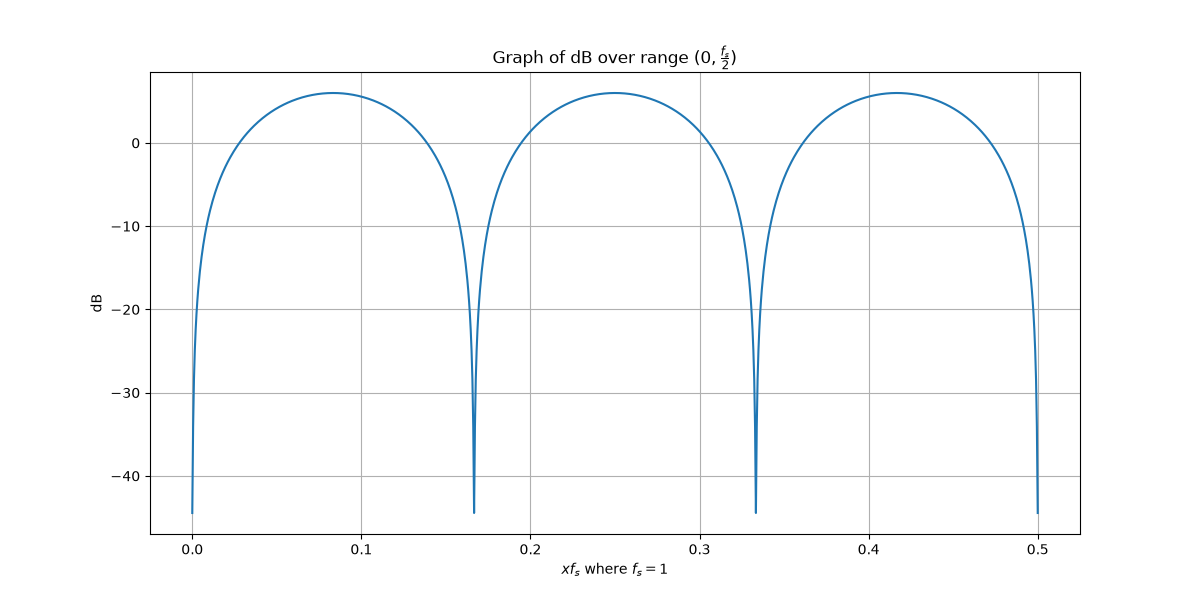
\includegraphics[width=\textwidth]{graph}
	\caption{Magnitude Response Graph in dB}
\end{figure}


\subsection{Phase response} \begin{align*}
	\freq{\omega}  & = 1 - R^L e^{-i L \omega}                                            \\
	\freq{\omega}  & = 1 - R^L (\cos(-L\omega) + i\sin(-L\omega))                         \\
	\freq{\omega}  & = (1 - R^L\cos(-L\omega)) + R^L i\sin(-L\omega)                      \\
	\theta(\omega) & = \arctan(\frac{-R^L \sin(L\omega)}{(1 - R^L\cos(L\omega))})         \\
	\theta(\omega) & = \arctan(\frac{-0.999^6 \sin(6\omega)}{(1 - 0.999^6\cos(6\omega))}) \\
\end{align*}

\section{Designing a Reson Filter}
One must first convert to radians per sample:
\begin{align*}
	f_s                 & = 44100 \si{\hertz}                                               \\
	B_{\si{\radian}}    & = 2\pi \frac{B_{\si{\hertz}}}{f_s}\ \si{\radian}/\text{sample}    \\
	\psi_{\si{\radian}} & = 2\pi \frac{\psi_{\si{\hertz}}}{f_s}\ \si{\radian}/\text{sample}
\end{align*}

Radians will be the default unit for the rest of the problem.

\subsection{With $B = 2 \phi,\ \cos\phi = 2 - \frac{1}{2}(R + \frac{1}{R})$}
\subsubsection{Deriving the pole radius formula}
\begin{align*}
	\phi     & = \frac{10\pi}{f_s}                \\
	\cos\phi & = 2 - \frac{1}{2}(R + \frac{1}{R}) \\
\end{align*}

Following the steps from class notes, one will obtain:
\begin{align*}
	0 & =R^2 - 2(2 - \cos\phi)R + 1                                         \\
	R & = \frac{2(2 - \cos(\phi)) \pm \sqrt{[-2(2 - \cos(\phi))]^2 - 4}}{2}
\end{align*}

\subsubsection{Evaluating with $B = 10 \si{\hertz},\ \psi = 1000 \si{\hertz}$}
Following the steps results in the filter:
\begin{align*}
	y_t \approx & 0.00020216605481176457x_t \\
	+           & 1.9783246236903536y_{t-1} \\
	-           & 0.998576255974041y_{t-2}
\end{align*}

The impulse response is the following:
\begin{align*}
	y_0 & = 0.00020216605481176457 \\
	y_1 & = 0.00039995008430844753 \\
	y_2 & = 0.00058935287793546
\end{align*}

\subsubsection{Evaluating with $B = 20 \si{\hertz},\ \psi = 5000 \si{\hertz}$}
Following the steps results in the filter:
\begin{align*}
	y_t \approx & 0.0018598988543063856x_t  \\
	+           & 1.511461125281618y_{t-1}  \\
	-           & 0.9971545393551153y_{t-2}
\end{align*}


The impulse response is the following:
\begin{align*}
	y_0 & = 0.0018598988543063856 \\
	y_1 & = 0.0028111648152399217 \\
	y_2 & = 0.002394359749681633
\end{align*}

\subsection{With approximation $B = 2(1 - R)$}
\subsubsection{Evaluating with $B = 10 \si{\hertz},\ \psi = 1000 \si{\hertz}$}
Following the steps results in the filter:
\begin{align*}
	y_t & = 0.0002022380575210094x_t \\
	+   & 1.978324121049828y_{t-1}   \\
	-   & 0.9985757489111912y_{t-2}
\end{align*}

The impulse response is the following:
\begin{align*}
	y_0 & = 0.0002022380575210094  \\
	y_1 & = 0.00040009242738807546 \\
	y_2 & = 0.00058956248000382
\end{align*}

\subsubsection{Evaluating with $B = 20 \si{\hertz},\ \psi = 5000 \si{\hertz}$}
Following the steps results in the filter:
\begin{align*}
	y_t & = 0.0018612234956407x_t   \\
	+   & 1.5114595871848688y_{t-1} \\
	-   & 0.9971525127908784y_{t-2}
\end{align*}

The impulse response is the following:
\begin{align*}
	y_0 & = 0.0018612234956407    \\
	y_1 & = 0.002813164096379871  \\
	y_2 & = 0.0023960601582540676
\end{align*}

\subsection{Comment}
They are suprisingly closer than I expected, it makes sense it's so widely used.

\section{Filter Reverse Engineering}
$$
	y_t = \sqrt{2}(0.99^t)\sin(\frac{\pi}{4}(t+1))
$$

This filter can be matched with the formula:
$$
	y_t = R^t[\frac{\sin(\theta(t+1))}{\sin\theta}]
$$

From there we can get the following:
\begin{align*}
	R      & = 0.99          \\
	\theta & = \frac{\pi}{4}
\end{align*}

\section{$R \approx e^{-\frac{B}{2}}$ Approximation Derivation}

% TODO: Finish this excercise

\section{Discrepancies of pole angles and peak frequencies}

% TODO: Finish this excercise

\end{document}
